\documentclass[12pt]{article}

\usepackage{epsfig}
\usepackage{pstricks}
\usepackage{pst-node}
\usepackage{a4wide}
\usepackage{amsmath}

\setlength{\oddsidemargin}{-2.5cm}
\setlength{\textwidth}{19cm}
\pagestyle{empty}

\newlength{\BIGlen}
\newcommand{\BIGL}[2][0cm]{
	\setlength{\BIGlen}{#1} \divide\BIGlen by 2
	$\left\}\text{ \rule[-\BIGlen]{0cm}{#1}#2}\right.$}

\newcommand{\BIGR}[2][0cm]{
	\setlength{\BIGlen}{#1} \divide\BIGlen by 2
	$\left\{\text{ \rule[-\BIGlen]{0cm}{#1}#2}\right.$}

\begin{document}

	\begin{pspicture}(19.5,19)
		\sffamily
		\psset{linewidth=0.5pt,fillstyle=solid,framesep=0,framesize=2.5 1}

		% lower box
		\psframe[linestyle=dotted,linewidth=1pt](0,0.5)(19.5,11)
		
		% description boxes
		\multips(1.5,7)(4.5,0){4}{\psframe(3.5,3.5)}
		\multirput[b](3.25,10.5)(13.5,0){2}{Description}
		
		\pnode(4.3,10.8){D1a}
		\pnode(4,7){D1b}
		\rput(3.25,8.75){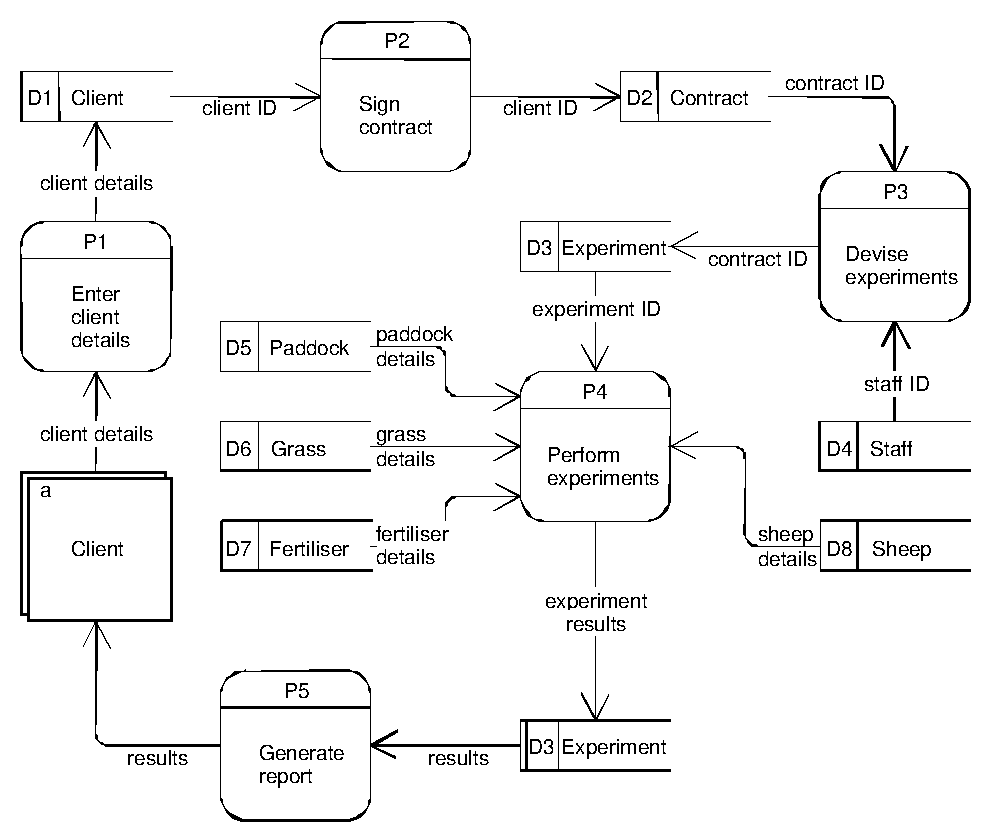
\epsfig{file=AgriDFD.eps,width=3cm}}

		\rput[b](7.75,10.5){\rnode{D2a}{Description}}
		\pnode(8,7){D2b}
		\rput(7.75,8.75){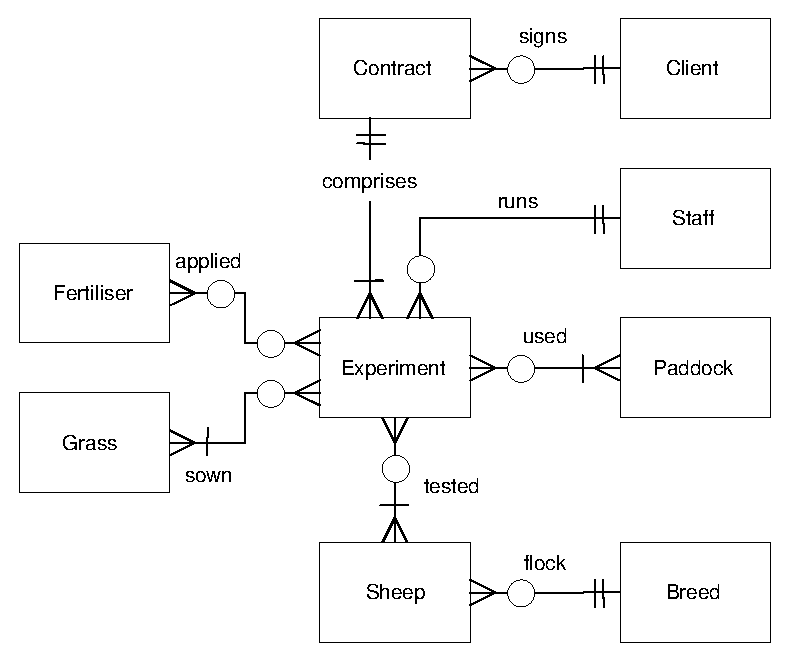
\epsfig{file=AgriERD.eps,width=3cm}}

		\rput[b](12.25,10.5){\rnode{D3a}{Description}}
		\pnode(11.25,7){D3b}
		\rput(12.25,8.75){\epsfig{file=AgriSQL.eps,width=3cm}}  % FIX THIS

		\pnode(15.7,10.8){D4a}
		\pnode(16,7){D4b}
		\rput(16.75,8.75){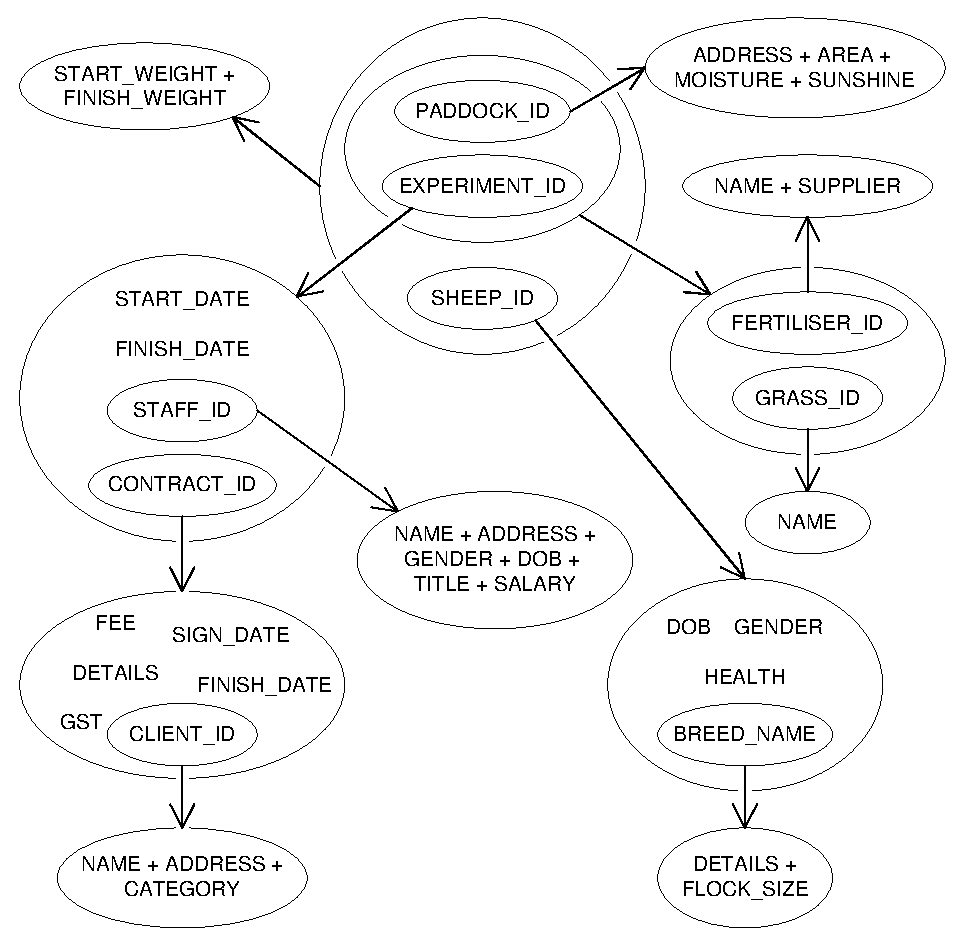
\epsfig{file=AgriFDD.eps,width=3cm}}
		
		\rput[t]{90}(18.6,8.75){elements}
		
		
		% representation boxes
		\multips(2.5,1)(4,0){4}{\psframe(3,4)}
		\multips(2.5,2.5)(4,0){4}{\psline(3,0)}
		\multips(2.5,4.5)(4,0){4}{\psline(3,0)}
		
		% DFD
		\pnode(4,5.5){R1}
		\rput[b](4,5){Representation}
		\rput(4,4.75){Proc. modelling}
		\rput[tl](2.6,4.4){\small \emph{Process}}
		\rput[r](5.4,3.75){\small \emph{Data flow}}
		\rput[b](3.5,3.1){\small \emph{Data store}}
		\rput(4,2.75){G\&S DFD}
		\psframe[framearc=0.1,fillstyle=none](2.75,1.875)(3.25,2.375)
		\psline(2.75,2.25)(3.25,2.25)
		\psline{->}(4,2)(5,2)
		\psline(4,1.5)(3.25,1.5)(3.25,1.125)(4,1.125)
		\psline(3.375,1.5)(3.375,1.125)
		
		% ER
		\pnode(8,5.5){R2}
		\rput[b](8,5){Representation}
		\rput(8,4.75){ERM}
		\rput[tr](9.4,4.4){\small \emph{Weak entity}}
		\rput[l](6.6,3.75){\small \emph{Attribute}}
		\rput[br](9.4,3.1){\small \emph{Relationship}}
		\rput(8,2.75){Martin ERD}
		\psframe[doubleline=true,fillstyle=none](8.5,1.75)(9.25,2.25)
		\rput[l](6.6,1.75){\small \texttt{emp\_no}}
		\pscircle(8.25,1.25){0.125}
		\psline(9,1.375)(9,1.125)
		\psline(9.25,1.375)(9.125,1.25)(9.25,1.125)
		\psline(8,1.25)(9.25,1.25)
		
		% Relational
		\pnode(11.25,5.5){R3}
		\multirput[b](11.25,5)(1.5,0){2}{Rep'n}
		\rput(12,4.75){Relational}
		\rput[tl](10.6,4.4){\small \emph{Primary key}}
		\rput[r](13.4,3.75){\small \emph{Attribute}}
		\rput[bl](10.6,3.1){\small \emph{Table}}
		\rput(11.25,2.75){SQL}
		\rput(11.25,1.75){\epsfig{file=SQLConstructs.eps,width=1.4cm}}
		\rput(12.75,2.75){QUEL}
		
		% FDD
		\pnode(16,5.5){R4}
		\rput[b](16,5){Representation}
		\rput(16,4.75){Functional Dep.}
		\rput[tr](17.4,4.4){\small \emph{Attribute}}
		\rput[l](14.6,3.75){\small \emph{Attribute set}}
		\rput[br](17.4,3.1){\small \emph{Dependency}}
		\rput(16,2.75){Smith FDD}
		\rput[tr](17.4,2.4){\small EMP\_NO}
		\rput(15.25,1.75){\psovalbox{\small A+B}}
		\psline{->>}(17.25,1.25)(16,1.25)
		
		\rput[t]{90}(17.6,4){\small \shortstack{``generic'' \\ constructs}}
		\rput[t]{90}(17.6,2){\small \shortstack{``specialised'' \\ constructs}}
		\psline[linewidth=1pt,linestyle=dashed,linecolor=gray](0.5,3)(18.75,3)
		\psline[linewidth=1pt,linestyle=dashed,linecolor=gray](12,3)(12,0.75)

		% viewpoint boxes
		\psframe[linestyle=dotted,linewidth=1pt](4.875,12)(15.125,13.5)

		\fnode(6.375,12.75){V1}
		\rput(6.375,12.75){Viewpoint}
		
		\fnode(10,12.75){V2}
		\rput(10,12.75){Viewpoint}

		\fnode(13.625,12.75){V3}
		\rput(13.625,12.75){Viewpoint}
		
		% perspective boxes
		\fnode(7,15){P1}
		\rput(7,15){Perspective}

		\fnode(10,15){P2}
		\rput(10,15){Perspective}

		\fnode(13,15){P3}
		\rput(13,15){Perspective}
		

		\psset{arrows=->,arrowscale=2,framesep=1pt}
		\rmfamily\small
		
		% arrows: descriptions to representations
		\ncline{D1b}{R1}\ncput*[npos=0.4]{expressed using}
		\ncline{D2b}{R2}\ncput*[npos=0.4]{expressed using}
		\ncline{D3b}{R3}\ncput*[npos=0.4]{expressed using}
		\ncline{D4b}{R4}\ncput*[npos=0.4]{expressed using}
		
		% arrows: viewpoints to descriptions
		\ncline{V2}{D1a}
		\ncline[nodesepB=0.1]{V2}{D2a}
		\ncline[nodesepB=0.1]{V2}{D3a}
		\ncline{V2}{D4a}
		
		% arrows: viewpoints to viewpoints
		\ncline{<->}{V1}{V2}
		\ncline{<->}{V2}{V3}
		
		% arrows: perspectives to viewpoints
		\ncline{P1}{V1}
		\ncline{P2}{V2}\ncput*[npos=0.375]{formalised as a}
		\ncline{P3}{V3}
		
		% arrows: real-world blob to perspectives
		\pnode(8.5,17.5){RWP1}
		\pnode(10,17.5){RWP2}
		\pnode(11.5,17.5){RWP3}
		\ncline{RWP1}{P1}
		\ncline{RWP2}{P2}\ncput*[npos=0.625]{viewed from several}
		\ncline{RWP3}{P3}
		
		% add other text labels
		\rput*[tl](0,0.4){\emph{Information system design environment using multiple modelling representations}}
		\rput*(10,11.5){described by one or more}
		\rput[r](1.9,2){\emph{scheme}}
		\rput[r](2.5,2){\BIGR[1.7cm]{}}
		\rput[r](1.9,4){\emph{technique}}
		\rput[r](2.5,4){\BIGR[1.7cm]{}}
		
		% phenomenon blob
		\rput(10,17.75){\input{::RWPBlob.tex}}%
		\rput(10,17.625){\large \textsf{\textbf{Real-world phenomenon}}}
		
	\end{pspicture}

\end{document}
